\documentclass{article}

\usepackage{tikz}
\usetikzlibrary{automata, positioning}
\begin{document}
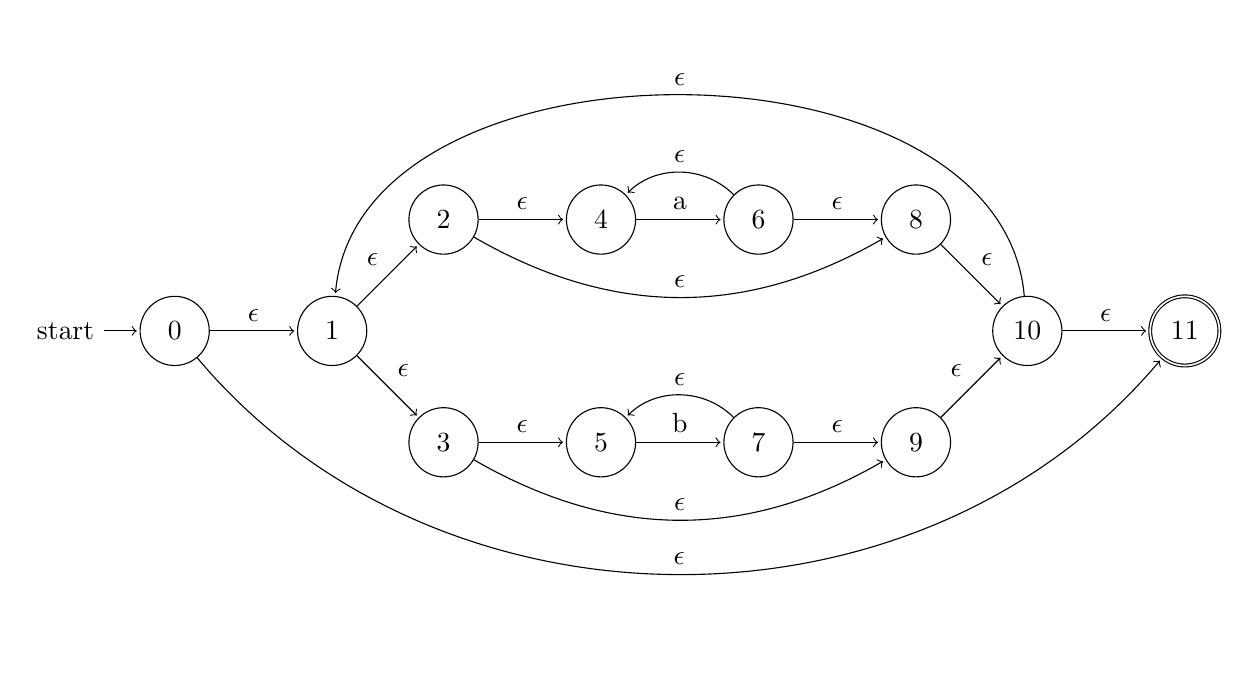
\begin{tikzpicture}[shorten >= 1pt, node distance = 2.0cm, on grid, auto]
  \node[state, initial] (0) {0};
  \node[state] (1) [right=of 0] {1};
  \node[state] (2) [above right=of 1] {2};
  \node[state] (3) [below right=of 1] {3};
  \node[state] (4) [right=of 2] {4};
  \node[state] (5) [right=of 3] {5};
  \node[state] (6) [right=of 4] {6};
  \node[state] (7) [right=of 5] {7};
  \node[state] (8) [right=of 6] {8};
  \node[state] (9) [right=of 7] {9};
  \node[state] (10) [below right=of 8] {10};
  \node[state, accepting] (11) [right=of 10] {11};
  \path[->]
    (0) edge node {$\epsilon$} (1)
        edge [bend right=50] node {$\epsilon$} (11)
    (1) edge node {$\epsilon$} (2)
        edge node {$\epsilon$} (3)
    (2) edge node {$\epsilon$} (4)
        edge [bend right] node {$\epsilon$} (8)
    (3) edge node {$\epsilon$} (5)
        edge [bend right] node {$\epsilon$} (9)
    (4) edge node {a} (6)
    (5) edge node {b} (7)
    (6) edge node {$\epsilon$} (8)
        edge [bend right=45] node [above] {$\epsilon$} (4)
    (7) edge node {$\epsilon$} (9)
        edge [bend right=45] node [above] {$\epsilon$} (5)
    (8) edge node {$\epsilon$} (10)
    (9) edge node {$\epsilon$} (10)
    (10) edge node {$\epsilon$} (11)
         edge [bend right=85] node [above] {$\epsilon$} (1);
\end{tikzpicture}

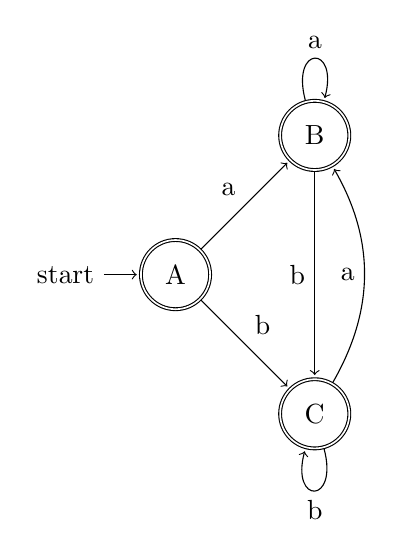
\begin{tikzpicture}[shorten >= 1pt, node distance = 2.5cm, on grid, auto]
  \node[state, initial, accepting] (A) {A};
  \node[state, accepting] (B) [above right=of A] {B};
  \node[state, accepting] (C) [below right=of A] {C};
  \path[->]
    (A) edge node {a} (B)
        edge node {b} (C)
    (B) edge node [left] {b} (C)
        edge [loop above] node {a} (B)
    (C) edge [bend right] node {a} (B)
        edge [loop below] node {b} (C);
\end{tikzpicture}
\end{document}
